\documentclass[authoryear, 12pt,5p, times]{elsarticle}
%\usepackage[hypcap]{caption}
%\geometry{margin=0.95in,top=1.4in,bottom=1.4in}
\geometry{margin=1.1in,top=1.5in,bottom=1.5in}
\usepackage{float}
\usepackage{amsmath}
\usepackage[hidelinks]{hyperref} 
 \usepackage{gensymb}
\usepackage{subcaption}
\usepackage{url}
%\renewcommand\thefootnote{\fnsymbol{\dagger}}
\usepackage[symbol*]{footmisc}
\makeatletter
\newcommand{\rpm}{\raisebox{.3ex}{$\scriptstyle\pm$}}
\begin{document}
\begin{frontmatter}
\title{Lab 8 : Op Amps III}
\author{\today \quad \\Jung Lin (Doris) Lee [Lab Partner: Leah Tom]\\Prof. William Holzapfel, GSI Thomas Darlington, Thomas Mittiga, John Groh,  \\Victoria Xu, Jonathan Ma, Francisco Monsalve, Xiaofei Zhou\vspace{-45pt}}	 
\end{frontmatter}
\section*{Introduction\label{intro}}
In our final lab on op amps, we investigate how op amps can deviate from its expected behavior to the golden rules. We investigate common imprefections in op amp circuits such as distortions and noises. In addition, we learn how a bipolar junction transistor (BJT) works  and how they can be used in circuits. We use circuit simulation programs to learn about how noise is generated and analyze the AC behavior of the components. Most importantly, we learn how these imperfections can be eliminated or alleviated in order to attain a $T_2$ audio signal with good sound quality.
 \section*{8.1}
 \begin{figure}[h!]
 \centering
 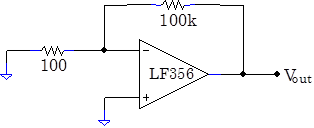
\includegraphics[width=0.5\textwidth]{figure/8_1_schema.png}
\caption{Circuit Schematic for the inverting amplifier}
\label{8_1_schema}
 \end{figure}
We built the inverting amplifier as shown in Fig.\ref{8_1_schema}  and measured the output voltage. We computed the input offset voltage by: 
\begin{equation}
V_{os}  = \frac{-10.8}{1000}  = 0.0108 V
\end{equation} To see whether this varies greatly for different op-amps, we conducted the same measurements for four other op amps, and obtained a $V_{out}$ of 452 $\pm$ 0.074 mV , 1.28 $\pm$ 0.0081536 mV,-1.03 $\pm$ 0.0081236 mV, and 1.08 V $\pm$ 0.3296mV. There is order-of-magnitude variations in the offset voltage of different op amps.
 \section*{8.2}
 We built the Fig.\ref{8_2_schema} circuit for removing the input offset.  Using the op-amp from question 1 which had an input offset voltage of 1.08m, we know that it has a corresponding $V_{out}$ of 1.08V. We adjusted the potentiometer until the scope reads a $V_{out}$ value of 2.24mV $\pm$0.04mV. After adjusting, the output was observed to drift between 1.88mV and 6.74mV. A possible reason for the drift could be due to an unsteady power supply or noise from the environment. 
  \begin{figure}[h!]
 \centering
 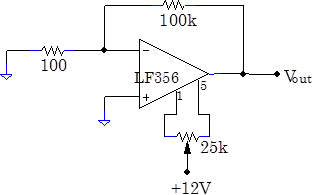
\includegraphics[width=0.5\textwidth]{figure/8_2_schema.png}
\caption{Circuit Schematic for removing input offset.}
\label{8_2_schema}
 \end{figure}
 \section*{8.3}
   \begin{figure}[h!]
 \centering
 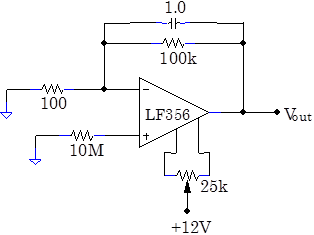
\includegraphics[width=0.4\textwidth]{figure/8_3_schema.png}
\caption{Circuit Schematic for measuring the input current bias.}
\label{8_3_schema}
 \end{figure}
We construct the circuit as shown in Fig.\ref{8_3_schema}.  When we short the 10M$\Omega$ resistor, the minimum $V_{out}$ measured is 1.88mV$\pm$ 0.04mV. When we removed the shorting wire, we measured a mean voltage of -120mV$\pm$0.05mV. The output voltage is a periodic wave with V$_{pp}$= 320mV. The input bias current ($I_B$)is computed as: 
 \begin{equation}
  I_B = \frac{\Delta V}{10M\Omega}=-1.22\times10^{-8} A  (3 s.f.)
\end{equation}  
 \section*{8.4}
 We drove the follower shown in Fig.\ref{8_4_schema} with a 10 V$_{pp}$, 1kHz triangular wave. We tried using different values of $R_L$ and found that as we increase the resistance the output current increases, so the output current does depend on the load resistance. The output current reaches a maximum when the resistance is around 5k$\Omega$. In looking at the scope traces, we found that at low resistance, the wave is more distorted than at high resistance. 
  \begin{figure}[h!]
 \centering
 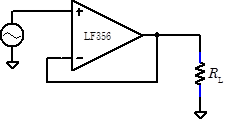
\includegraphics[width=0.5\textwidth]{figure/8_4_schema.png}
\caption{Circuit Schematic for the inverting amplifier}
\label{8_4_schema}
 \end{figure}
  \section*{8.5}
 We built the amplifier as shown in Fig.\ref{8_5_schema}. Feeding in different functional waveforms as $V_{in}$ with $V_{pp}$ as 1.00 V and a frequency of 1lHz, we find  that the sine wave has the lowest pitch, and the square wave  sounds slightly higher. The triangular wave has a distinguisahbly much higher pitch and sounds sharp to the ear.
  \begin{figure}[h!]
 \centering
 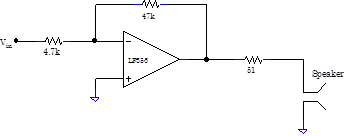
\includegraphics[width=0.5\textwidth]{figure/8_5_schema.png}
\caption{Circuit Schematic for the audio amplifier.}
\label{8_5_schema}
 \end{figure}
 \par The maximum amplitude that we can drive the speaker without distortion is 320.0 m$V_{pp}$. The volume lowers when we decrease the amplitude. Using the $T_2$ audio output, we obtained a sound of acceptable quality but not of the clearest sound quality.
 \section*{8.6}
 Using a sine wave input, we find that the volume increased as we increased the input amplitude from 0.01 to 1V. When the amplifier is driven by T2, the sound quality is poor. The speaker only emits a pure sine note at 20m$V_{pp}$ as observed from the scope traces. Sketches of the output waveforms as shown in Fig.\ref{lotsofwaves}.  As the amplitude is increases, the output waveform becomes more distorted and the lower part of the sine wave gets more rectified. 
  \begin{figure*}[h!]
  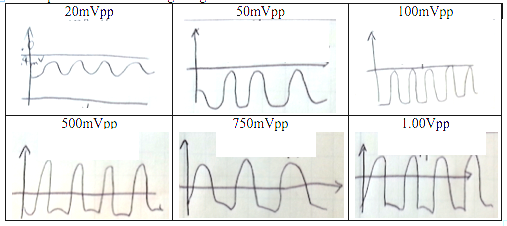
\includegraphics[width=\textwidth,height=6cm]{figure/waveformlots.png}
\caption{Sketches of output waveforms with corresponding input amplitudes.}
\label{lotsofwaves}
\end{figure*}
 \section*{8.7}
 We try to improve the follower's performance by including a feedback loop in the circuit, so that it takes a larger input amplitude to distort the waveform. In this circuit, sine wave gets distorted beyond input amplitude of 270m$V_{pp}$. The circuit can amplifying triangular waves without distortion as shown in Fig.\ref{8_7_scope} with a tolerance of a higher amplitude. On the other hand, we find that the square wave gets distorted and exhibits sharp peaks when the signal's sign changes, while retaining the general waveform of a square wave.
   \begin{figure*}[h!]
  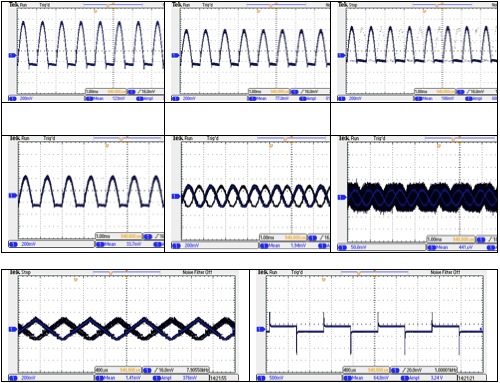
\includegraphics[width=\textwidth,height=6cm]{figure/8_7_scope.png}
\caption{Sketches of output wave forms arranged with increasing input amplitudes towards the right. Top row features the triangular wave which is rectified but not distorted. Middle row shows the increasing distortion as amplitude is increased for the sinusoidal waveform. Likewise, the bottom row shows distortion for the square waveform.}
\label{8_7_scope}
\end{figure*}
 \section*{8.9}
 \begin{figure}[h!]
 \centering
  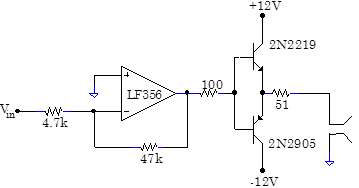
\includegraphics[width=0.5\textwidth]{figure/8_9_schema.png}
\caption{Circuit Schematic of the follower circuit.}
\label{8_9_schema}
 \end{figure}
\par  We built the circuit shown in Fig. \ref{8_9_schema}and fed in a 500 Hz sine wave of different amplitudes. As shown in the scope traces in Fig.\ref{crossover} , we find that the cross over distortion near the x axis is most evident in the 0.15 and 1.5 V$_{pp}$ cases. We also find that the cross over distortion is more evident at very high frequencies, since the transistor is out of its operating range.
 \begin{figure*}[h!]
  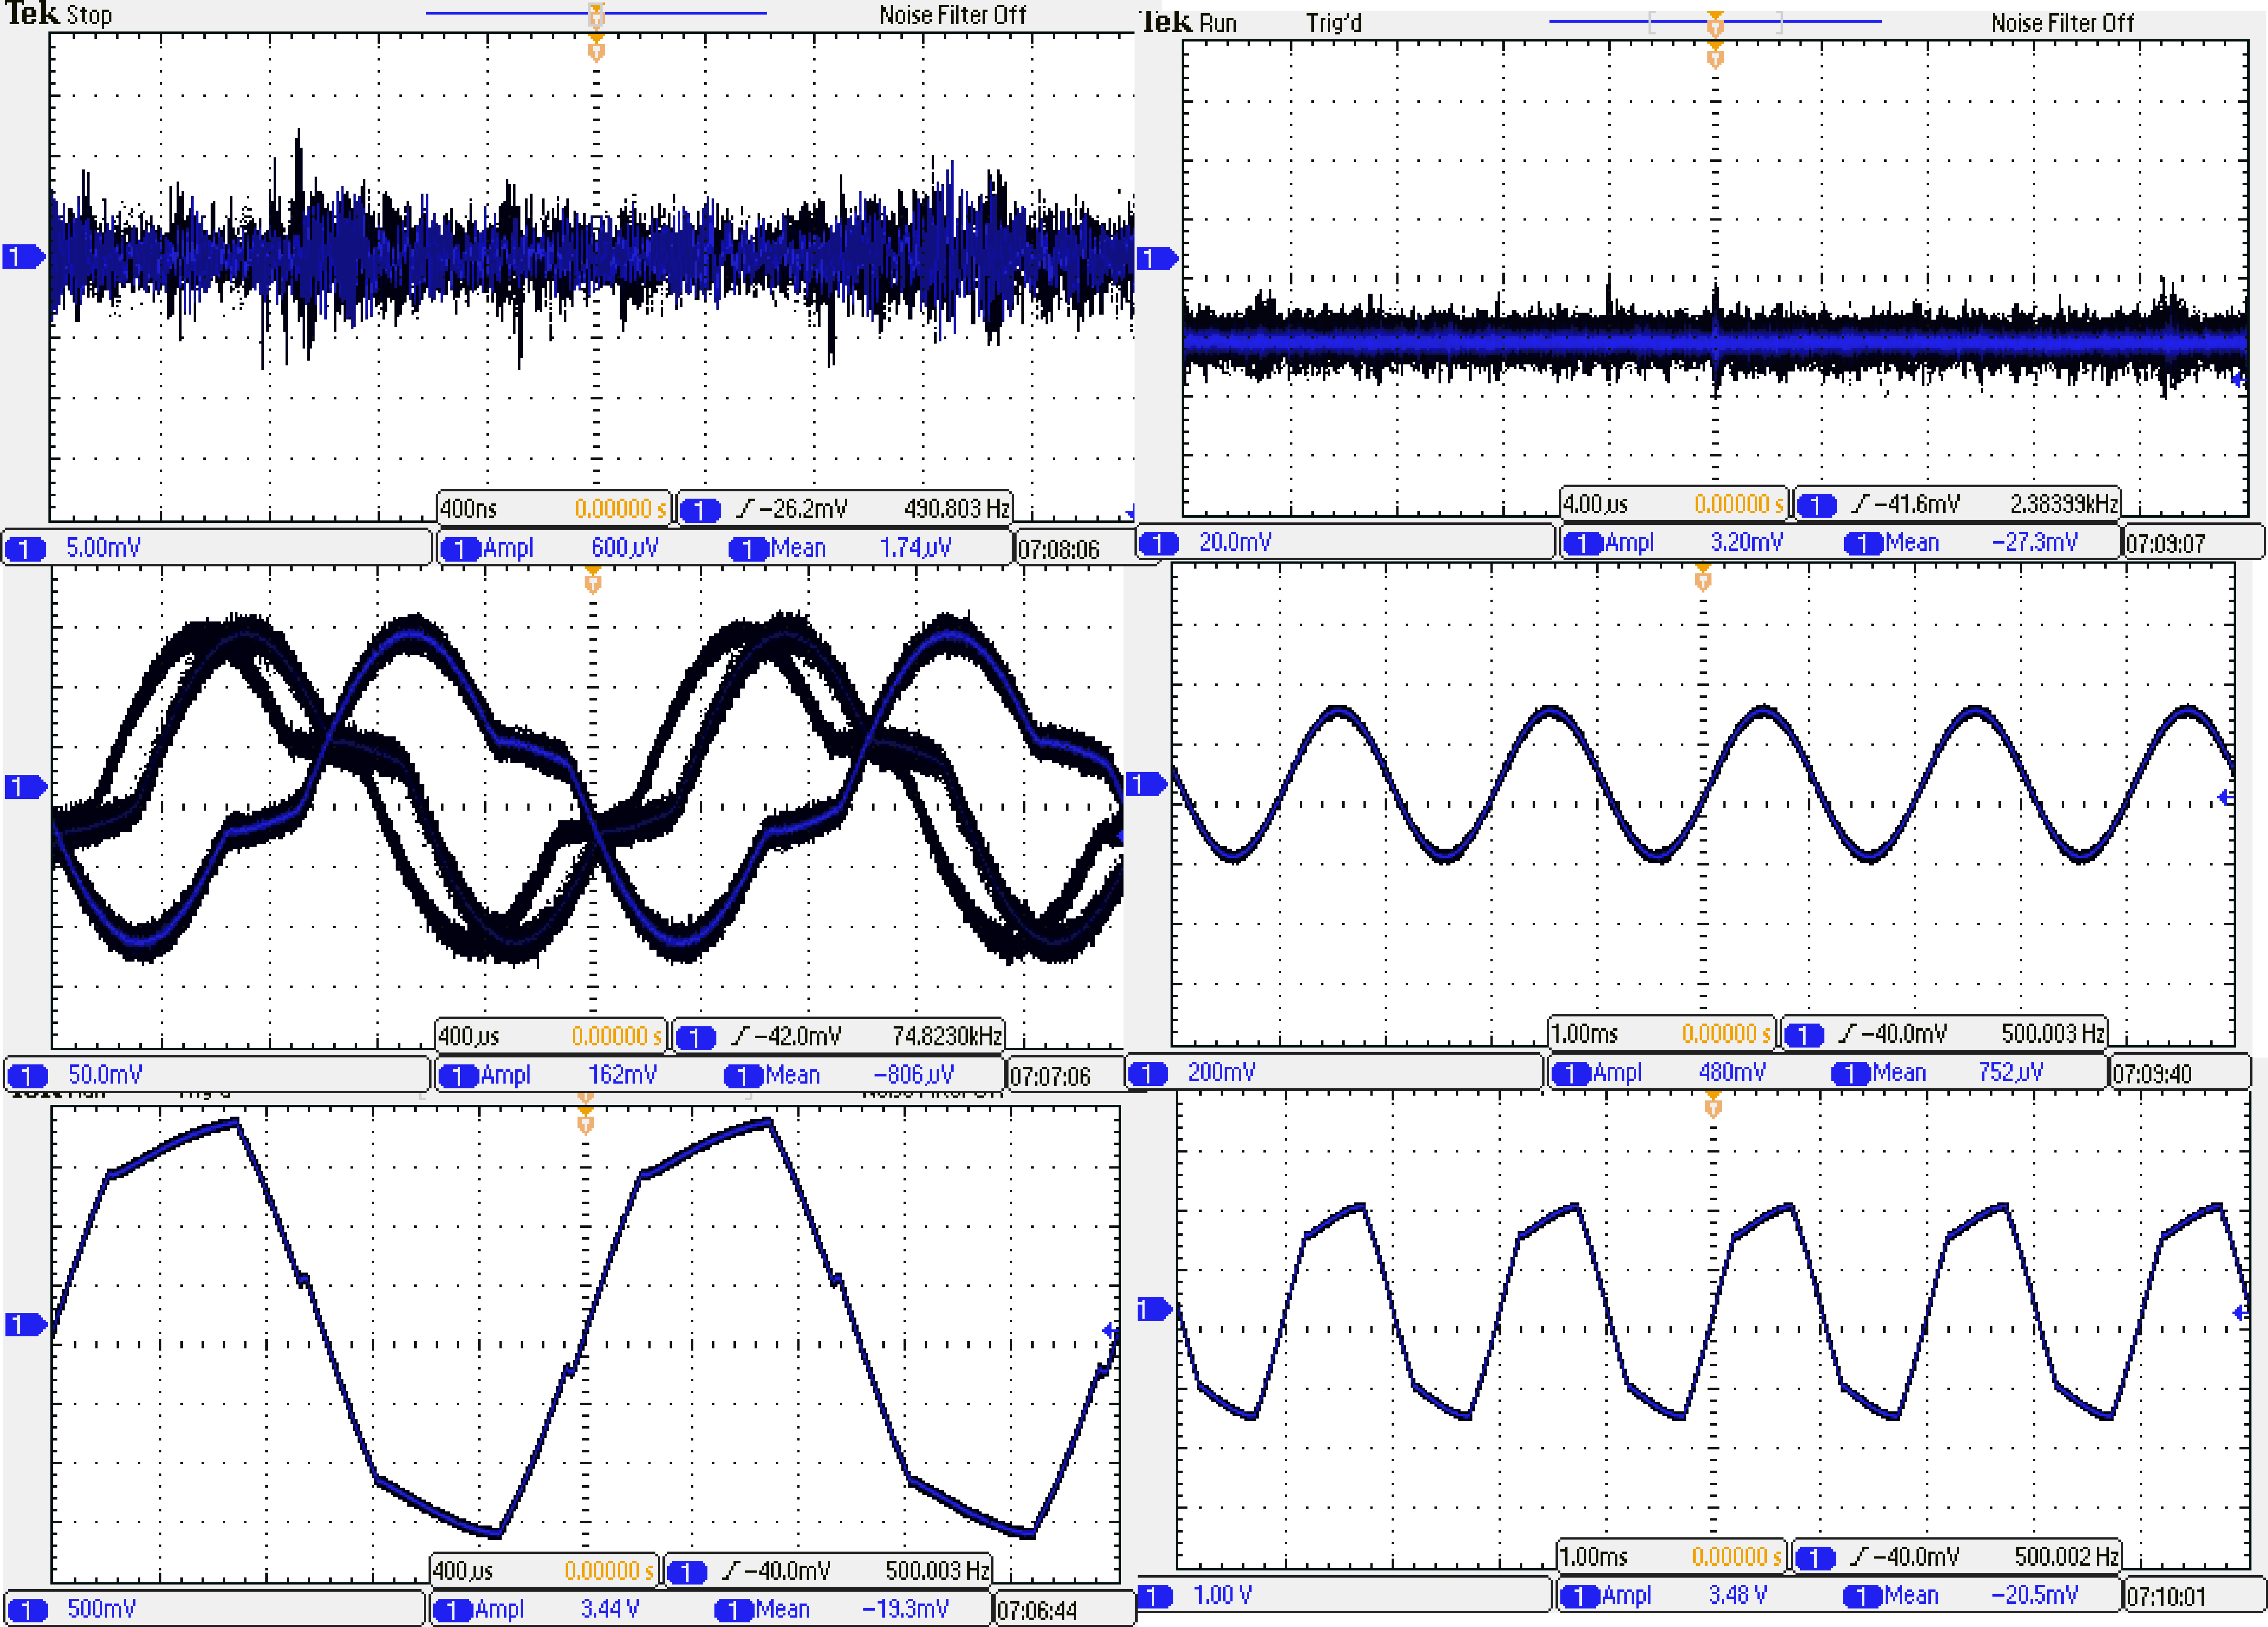
\includegraphics[width=\textwidth,height=6cm]{figure/crossover_scope.png}
\caption{Crossover distortion in for an input wave amplitude of 0.015 (Top) ,0.15 (Middle) and 1.5 V$_{pp}$(Bottom). The left panels show the signal behaviour for the Fig.\ref{8_9_schema} circuit, right panels for the second circuit in Fig. \ref{8_9_schema2}.}
\label{crossover}
\end{figure*}
 \par Crossover distortion happens when the signal goes from one device to another. In Fig.\ref{8_1_schema}, the signal crosses over from the upper BJT to the lower BJT. For the top BJT  the voltage across the base and emmiter (V$_{BE}$) is a nonzero value, so the signal will not go through unless the input signal is smaller than V$_{BE}$. Likewise, this also happens when the upper transistor stops passing through current and the current goes through the lower portion and also feeds to the load (50$\Omega$ resistor and speaker). Therefore,  in the V=0 region the transition stops at a value to the right and left of the original zero point, resulting in the ``kink" in the crossover region.  
 \par Then, we change the connection of the 47k$\Omega$ to be on the node leading the 51$\Omega$ resistor that protects the speaker, as illustrated in Fig. \ref{8_9_schema2}.
 \begin{figure}[h!]
 \centering
  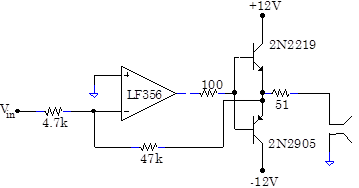
\includegraphics[width=0.5\textwidth]{figure/8_9_schema2.png}
\caption{Circuit Schematic of push-pull feedback circuit.}
\label{8_9_schema2}
 \end{figure}
\par As evident from the scope traces in Fig. \ref{crossover}, we find that the crossover distortion is diminished when compared with the scope trace of the same amplitude settings. Using the T$_2$ audio signal, we find that the sound quality is slightly better in the circuit in Fig.\ref{8_9_schema2}.
  \section*{8.11}
The generator still generates a Gaussian distribution everytime we do a generate spectrum because a inverse Fourier transform of a Gaussian function is still a Gaussian function, as shown in FIg.\ref{gaussian} . Uniform white noise sounds like the Gaussian noise, but the volume is slightly louder.  The 1/f noise does sound like a distant ocean wave, with a lower sound volume.
\begin{figure}[h!]
 \centering
 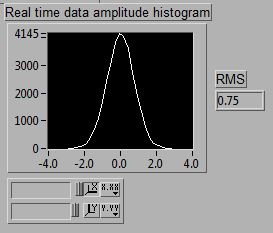
\includegraphics[width=0.5\textwidth]{figure/generate_spectrum.jpg}
\caption{Amplitude histogram of Gaussian noise.}
\label{gaussian}
 \end{figure}
\par We find that if we alter the low-pass frequency, it cuts away the high frequency noises. When we generate a spectrum as a superposition of many low frequency waves, then the audio rfequency sounds lower (like a furnace) since only the low frequencies below 500 Hz can pass through the filter as shown in the Fig. \ref{furnace}.
\begin{figure}[h!]
 \centering
 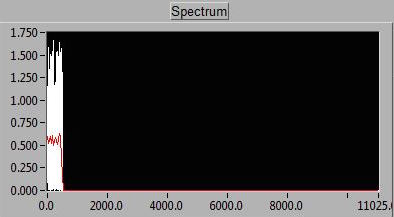
\includegraphics[width=0.5\textwidth]{figure/furnace.jpg}
\caption{Low pass frequency set as 500 Hz.}
\label{furnace}
 \end{figure}
 \par When the average number of shots per sample is set as 0.0010, the arrival time of the particle on the detector sounds discrete, like a popping sound of the radio when it is not tuned at a channel. We tried setting the average number to 
larger numbers and the sound became more continuous and sounding like Gaussian noise. This corresponds to the histogram shown in Fig.\ref{shot}
 \begin{figure}[h!]
 \centering
 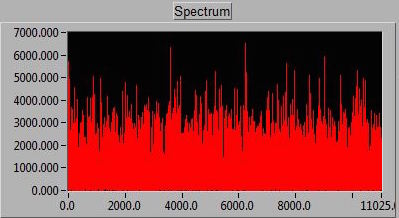
\includegraphics[width=0.5\textwidth]{figure/N_1000_shot_spectrum.JPG}
  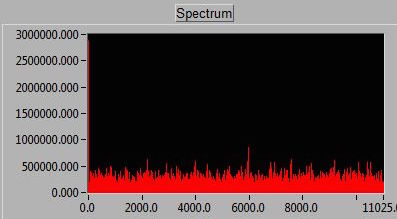
\includegraphics[width=0.5\textwidth]{figure/N_100000_shot_spectrum.JPG} 
\caption{The average number of shots per sample can be estimated from the y-axis as the mean of the spectrum. [x: frequency ; y: number of shots] }
\label{spectrum}
 \end{figure}
 \par In addition, as we increase the average number of shots, the volume also decreases because when there is greater number of peaks added up together. The superposition of the wave diminishes the variation of the waves (even though it provided a larger offset). Since amplitude measures the difference between the peak and trough of the wave, we volume decreases as we increase the average number of shots. 
 \begin{figure*}[h!]
  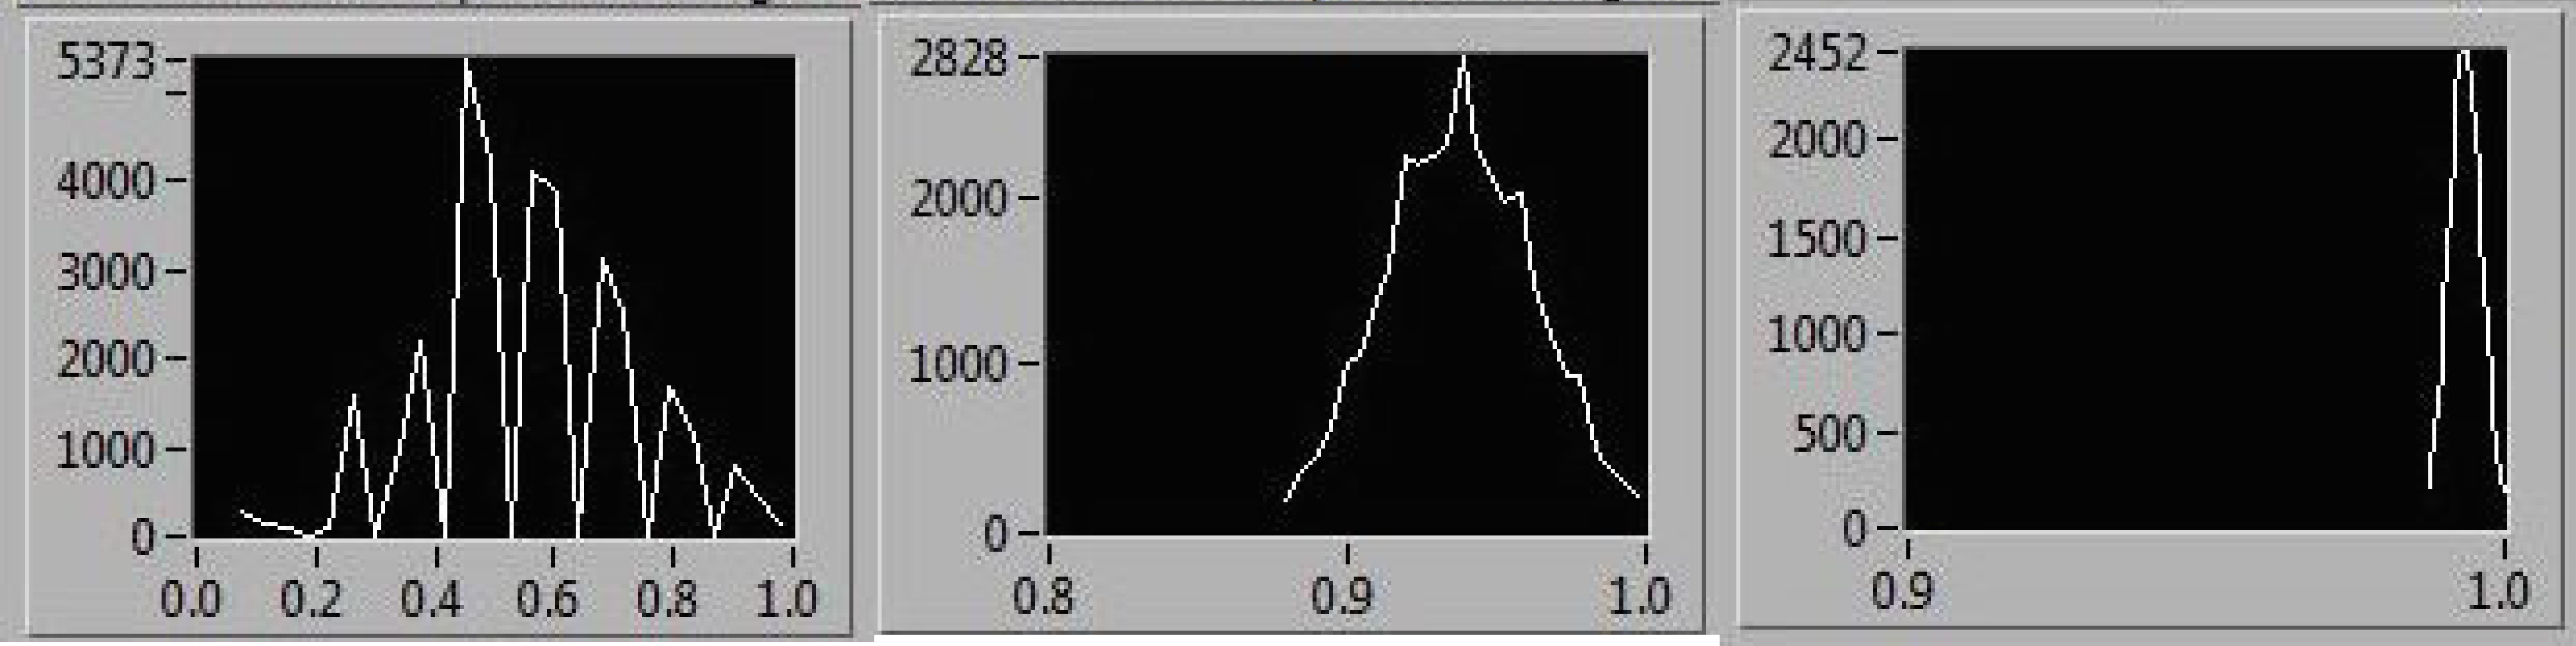
\includegraphics[width=\textwidth,height=4cm]{figure/shot.png}
\caption{Left: N = 10; Middle: N=1000 ; Right N=10000.  [Real-time data amplitude histogram; x: amplitudes ; y: counts] When we set the average number of shots per sample to larger numbers the spectrum looks more Gaussian and shifts towards the 1.0.}
\label{shot}
\end{figure*}

\par For the line noise, at low harmonic content, the sound is smooth, but begins to get noisy as harmonic content exceeds 0.8. This is because it is now composed of more frequency components, as shown in Fig.\ref{line}. The sound of the line noise sounds like the buzzing 60 Hz noise of common electronic appliances such as an old CRT TV monitor.
 \begin{figure*}[h!]
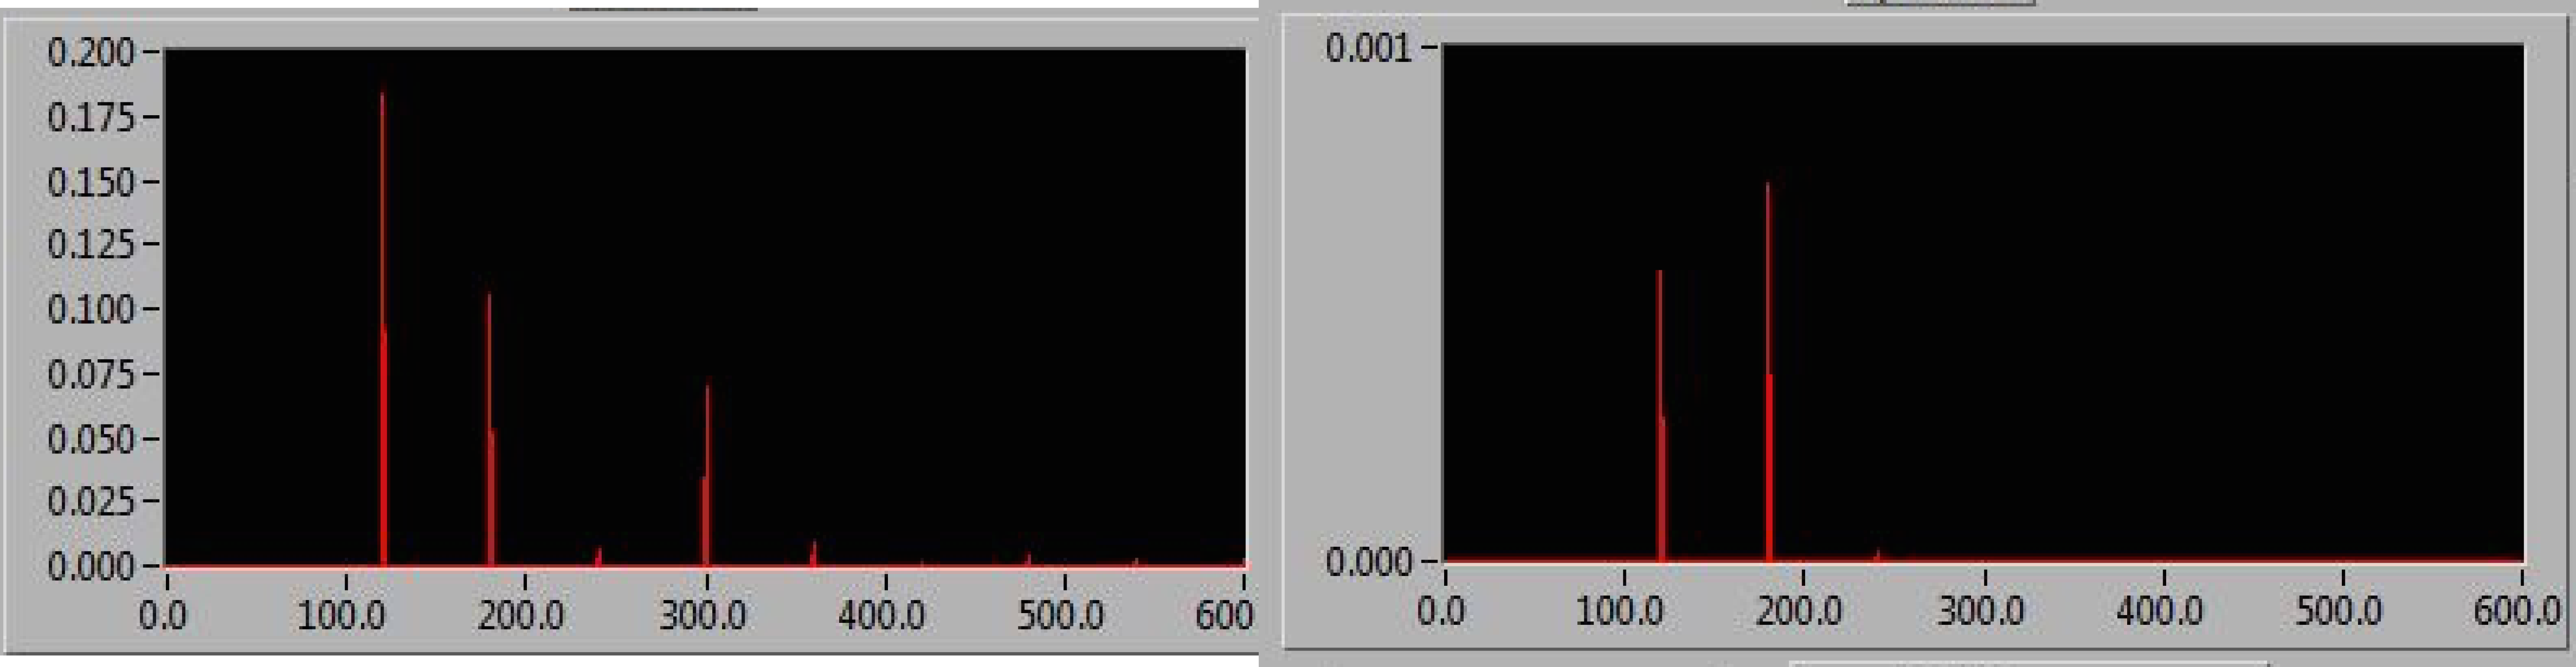
\includegraphics[width=\textwidth,height=4cm]{figure/line.png}
\caption{Decomposed spectrum for the noise signal. Left: Harmonic content 0.2; Right: Harmonic Content: 0.8 . [x: frequency ; y: number of shots] }
\label{line}
 \end{figure*}
\section*{8.12}
Using Multisim, we simulate the circuit shown in Fig. \ref{schema8_12}: 
 \begin{figure}[h!]
 \centering
  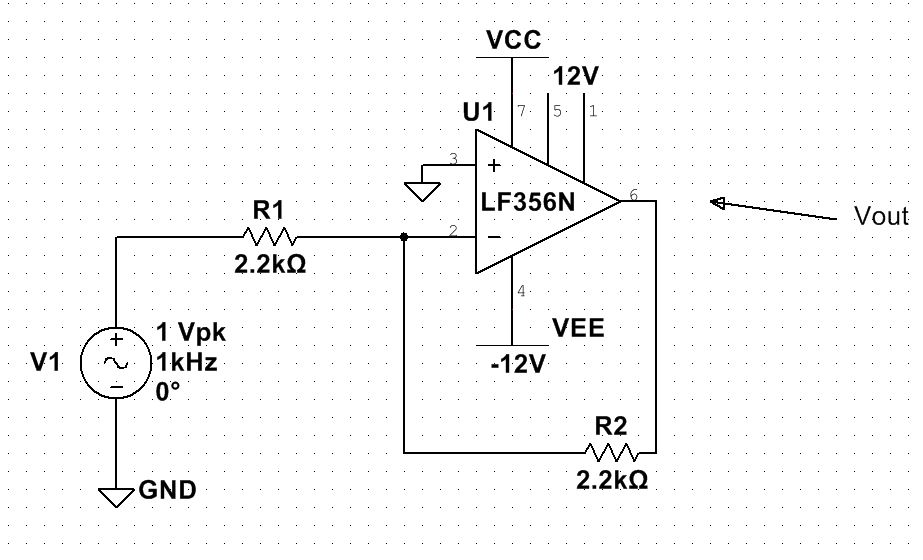
\includegraphics[width=0.5\textwidth]{figure/8_12_schematic.JPG} 
\caption{Circuit schematic}
\label{schema8_12}
 \end{figure}
We conduct a AC analysis by examining how the LF356 responds to different frequencies. We consider only the behavior in the frequency range of 0 to 100 kHz, (operating range of the op amp). From Fig.\ref{phase}, we subtract the difference between the V$_{out}$ and V$_{in}$ and obtained a phase shift of about 180 degrees. In the operating range, V$_{out}$ and V$_{in}$ are approximately equal so the gain is about one.
 \begin{figure}[h!]
 \centering
  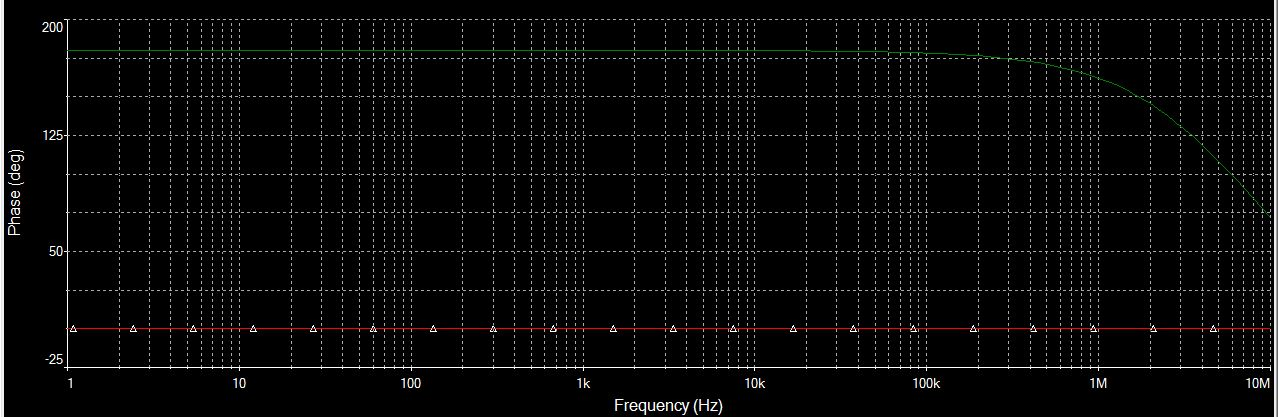
\includegraphics[width=0.5\textwidth]{figure/8_12_phase_shift.JPG} 
\caption{Frequency response of circuit based on $V_{out}/V_{2}$. Above: Magnitude plot. Below: Phase shift plot}
\label{phase}
 \end{figure}
 \section*{8.13}
 We constructed the differentiator as shown in Fig.\ref{8_13_schema}. By measuring the output signal on the oscilloscope, we find that the output waveform is sinusoidaal with a frequency of 2.23kHz. The sine wave is modulated by another wave with a lower frequency. Despite the grounded input and decoupled capacitors to prevent parasitic oscillation, the output signal still fluctuates greatly. 
 \begin{figure}[h!]
 \centering
  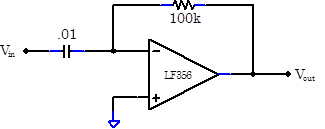
\includegraphics[width=0.5\textwidth]{figure/8_13_schema.png} 
\caption{Circuit Schematic for the differentiator.}
\label{8_13_schema}
 \end{figure}
\par This behaviour is explained by the fact that there there is a phase shift between the signal from ground to the input after passing through capacitor and the ground. To compensate this effect, V$_{out}$ has a phase shift from the input which creates potential difference, causing the oscillations we see in Fig.\ref{8_13_scope}. Because the capacitor introduces a $\pi/2$ phase shift between the input and output signal, the circuit is able to differentiate its input. Mathematically, the phase difference between a cosine and sine is $\pi/2$, so if we were to model the input wave as sine wave, then the output wave would be a cosine wave and vice versa. This yields a differentiated output signal. 
 \begin{figure}[h!]
 \centering
  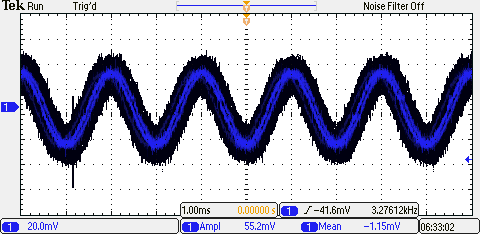
\includegraphics[width=0.5\textwidth]{figure/8_13_scope.png} 
\caption{Scope traces showing signal from a differentiator.}
\label{8_13_scope}
 \end{figure}
  \section*{8.14}
Compared to the differentiator in 8.13, this circuit is more stable and fluctuates to a lesser extent. This improvement is due to the addition of a capcitor between the input and output, which acts as a bypass filter for any oscillating signals in the background. When varying the frequencies and taking measurement on the oscilloscope, we obtained the transfer function and the phase difference as plotted in Fig.\ref{8_14_plot}.
 \begin{figure}[h!]
 \centering
  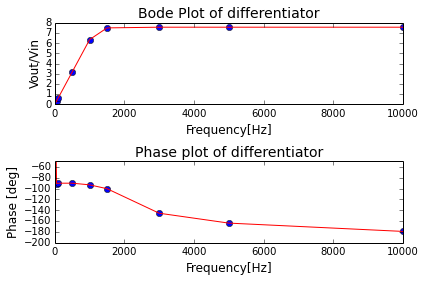
\includegraphics[width=0.5\textwidth]{figure/8_14_plot.png} 
\caption{Above: Bode plot of differentiator; Below: Phase difference plot. We find that the gain increases linearly between the range of 0 and 2Hz and then flattens out at around 5kHz. The circuit differentiates signals with frequencies between 0Hz and around 1400Hz.}
\label{8_14_plot}
 \end{figure}
 \section*{8.15}
We drove an op amp follower as shown in Fig. \ref{8_4_schema} . As shown in the scope trace in Fig.\ref{scope}, the slew rate is the maximum rate of change of output voltage per unit of time. We compute the slew rate as: 
\begin{equation}
 \frac{4 div \times 5.00V/div}{1.5 div \times 2.00 \mu s /div}
 = \frac{20.0V}{3.00\mu s} = 6.67 V/\mu s
\end{equation} 
 \begin{figure}[h!]
 \centering
  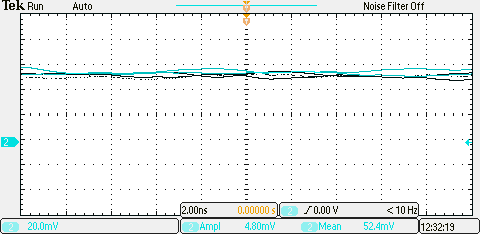
\includegraphics[width=0.5\textwidth]{figure/TEK00000.png} 
\caption{Scope trace for measuring slew rate of op amp follower.}
\label{scope}
 \end{figure}
\section*{8.19}
The gain of an inverting amplifier can be computed by : 
\begin{equation}
G = \Bigg |\frac{V_{out}}{V_+ - V_-}\Bigg |=\Bigg |\frac{V_{out}}{ V_-}\Bigg |
\end{equation} 
We consider the behavior of the circuit in question 8.12, and compute the gain and averaged the value over the frequency range $10^2$ to $10^7$ Hz and obtain a gain of around 5149. [NEED TO COMPARE WITH RESULTS IN 17!!!!!] 
\section*{Conclusion}
In this lab, we examine situations where the function of op-amps is limited and scenarios where the op-amp golden rules are violated. We investigate possible sources of errors such as Johnson noise and input bias currents. In addition, we continue to explore applications of op-amps by building advanced circuits such as the bipolar follower and the push-pull circuit.
 \section*{Acknowledgments}
\begin{footnotesize}
The author would like to acknowledge support from the GSI in this lab in addressing our questions about the lab and with the handling of liquid nitrogen. I would also like to thank my partner, Leah Tom, for helpful discussion and collaboration that helped this work. We also appreciate Alan Luu for providing us with guidance on question 8.18.
\end{footnotesize}
  \section*{References}
 \begin{footnotesize}
 \begin{itemize}
 \item Horowitz, Paul, and Winfield Hill. \textit{The Art of Electronics}. Cambridge: Cambridge UP, 1989. Print.
\item ``Crossover Distortion." \textit{Wikipedia}. Wikimedia Foundation, n.d. Web. 02 Apr. 2015.
 \item ``Lab 8 - Op Amps III." \textit{Donald A. Glaser Advanced Lab.} Regents of the University of California, n.d. Web. 29 Mar. 2015.
\end{itemize} 
  \end{footnotesize}

\end{document}
